\documentclass[a4paper,12pt]{article} 
 \sloppy

 % report, book

 % Рисунки
 \usepackage{graphicx}
 \DeclareGraphicsExtensions{.pdf,.png,.jpg}
 \usepackage{wrapfig}
 % Гиперссылки
 \usepackage{hyperref}
 \usepackage[rgb]{xcolor}

 %  Русский язык

 \usepackage[T2A]{fontenc} % кодировка
 \usepackage[utf8]{inputenc} % кодировка исходного текста
 \usepackage[english,russian]{babel}	% локализация и переносы
 \usepackage {indentfirst} % отступ
 \usepackage[left=2.5cm,right=2.5cm,
     top=2cm,bottom=2cm,bindingoffset=0cm]{geometry}

 % Кавычки
 \usepackage {csquotes}
 \DeclareQuoteStyle{russian}
     {\guillemotleft}{\guillemotright}[0.025em]
     {\quotedblbase}{\textquotedblleft}


 % Код
 \usepackage {listings}


 % Математика
 \usepackage{amsmath,amsfonts,amssymb,amsthm,mathtools} 
 \usepackage{biblatex}



 \usepackage{wasysym}
\title{Сопоставление изображений с помощью сиамских нейронных сетей}
\author{Шабанов Ахмедхан}
\date{}
\begin{document}
% \maketitle
% \section{Introduction}
Сопоставление (совмещение) изображений - важная задача компьютерного зрения, которая заключается в приведении двух или более изображений к общей системе координат.

Большинство методов сопоставления изображений можно разделить на два класса: плотные и разреженные. Плотные алгоритмы сопоставления находят похожие области сопоставляемых изображений, и при нахождении преобразования анализируются все пиксели, входящие в эти области. Разреженные методы находят сопоставление анализируя множество отдельных точек, как правило, “разбросанных” по всему изображению. Метод сопоставления изображений с помощью сиамских нейронных сетей относится к разреженному классу (но об этом позже). 

Разреженный подход, при котором принятие решения об искомом преобразовании осуществляет путем анализа и поиска соответствий между двумя наборами небольших участков изображений (“патчей”), состоит из трех основных шагов:
\begin{itemize}
    \item выделение подмножества устойчивых точек, совокупность которых позволяет идентифицировать и/или сопоставить изображения; 
     \item поиск пар устойчивых точек, соответствующих одной физической точке; 
     \item нахождение геометрического преобразования, переводящего устойчивые точки одного изображения в соответствующие устойчивые точки другого. 
\end{itemize}

Эти три шага показаны на рисунке \ref{graph}
\begin{figure}[!h]
     \centering
     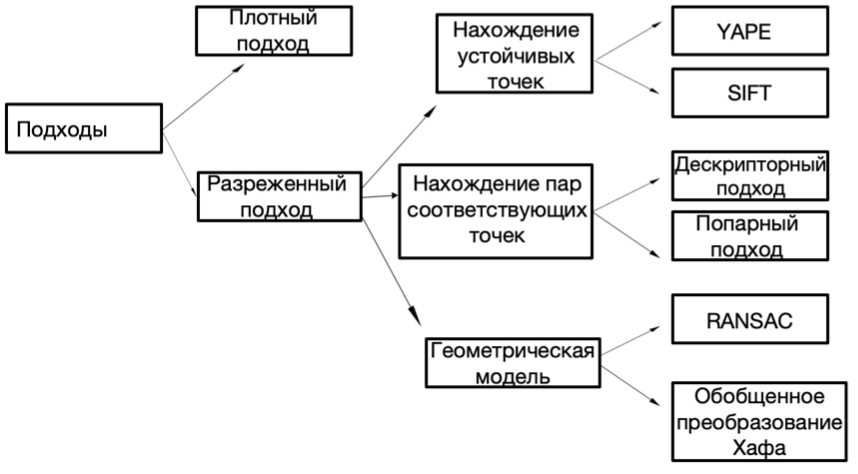
\includegraphics[width=130mm]{graph.png}
     \caption{Алгоритмы, используемые для сопоставления изображений}
     \label{models}
\end{figure}

В качестве детектора особых точек можно использовать следующие методы:  SIFT (Scale Invariant Feature Transfrom), SURF [20] (Speeded Up Robust Features) или YAPE (Yet Another Point Extractor) и так далее.

Для решения задачи сопоставления изображений разреженным методом, после нахождения устойчивых точек необходимо найти соответсветствие между устойчивыми точками двух изображений (то есть понять, какие пары устойчивых точек соответствут одной физической точке). Обычно, для этого анализируются некоторые окрестности рассматриваемых точек. Такие окрестности называются “патчами”. 

Алгоритмы, которые осуществляют поиск соответствий, можно разделить на два типа:
\begin{itemize}
    \item “Попарный подход”. В этом случае алгоритм получает на вход два патча - по одному с каждой из картинок. Выходом такого алгоритма является численная оценка схожести двух входных патчей.
    \item “Дескрипторный подход”. В этом случае алгоритм получает на вход только один патч. Выходом алгоритма является некоторый вектор. Решение о том, какие патчи соответствуют друг другу, принимается путем сравнения дескрипторов некоторой легко вычислимой метрикой (например, L1 или L2 норма).
\end{itemize}

В основе многих способов решения данной задачи с помощью нейронных сетей лежит сиамская нейронная сеть. Это такая сеть, которая принимает на вход 2 изображения, и обрабатывает их одинаковым способом (моделью с одинаковыми весами). На выходе получаем вектора, соответствующие входным изображениям.
Такая сеть может быть применена как в “Попарном подходе” так и в “Дескрипторном подходе”: 
\begin{itemize}
    \item Вектора на выходе модели можно воспринимать как дескрипторы входных изобрежений и учить модель так, чтоб евклидово расстояние между дескрипторами для “похожих” изображений было малым, а для “непохожих” - большим ( рисунок \ref{models} a).
    \item Вектора на выходе модели можно подать на вход другой модели, которая будет решать задачу бинарной классификации: 1 - входные изображения, которым в соответствие ставятся дескрипторы, “похожи”, 0 -  “непохожи” (рисунок \ref{models} b).
\end{itemize}
Алгоритмы сопоставления получают на вход два патча, и выдают степень их похожести. Однако, при решении задачи сопоставления обычно число возможных ребер намного превышает число устойчивых точек. При этом дескрибируемые патчи - маленькие куски изображений - как правило имеютбольшую избыточность, и перед их сравнением, зачастую, эффективно снизитьих размерность. Это позволит использовать вычислительно эффективный метод сопоставления патчей в пространстве уменьшенной размерности

Но в попарном подходе на вход второй (классифицирующей) модели можно подать дополнительную информацию о входных изобрежениях, которая может быть полезна для определения схожести. Например (как в модели hybrid approach на рисунке \ref{models} b), можно на вход модели так же подать значение кросс-корреляции между входными изображениями.

Общий алгоритм сопоставления двух изображений с помощью сиамской нейронной сети:

На вход подаются два изображения $I_{1}, I_{2}$, тип детектора, тип геометрической модели, семейство геометрических преобразований $\mathcal{T}$.
\begin{enumerate}
    \item Подалгоритм детектирования устойчивых точек. 
    
    На вход: два изображения $I_{1}, I_{2}$, тип детектора.
        \begin{itemize}
            \item С помощью заданного детектора находятся множества устойчивых точек $F_{1}$ и $F_{2}$. Обозначим $N_{1} = |F_{1}|$ и $N_{2} = |F_{2}|$ - число найденных точек на оптическом и радиолокационном изображении соответственно.
            \item На изображениях выделяются подизображения (патчи) размера $L$x$L$ с центром в найденных точках. Получаем множества патчей $P_{1}$ и $P_{2}$
        \end{itemize}
        На выходе: множества патчей двух изображений $P_{1}$ и $P_{2}$.
        
    \item Подалгоритм нахождения соответствующих пар точек.
    
    На вход: множества патчей двух изображений $P_{1}$ и $P_{2}$, множества устойчивых точек $F_{1}$ и $F_{2}$.
        \begin{itemize}
            \item Из всевозможных пар патчей $Pairs = \{ (\rho_{1}, \rho_{2}) | \rho_{1} \in P_{1}, \rho_{2} \in P_{2}\}$  оценивается подмножество соответствующих ($Corr\_patches$)  - такие патчи, центры которых соответствуют одной физической точке.
            \item Из найденных соответствующих пар патчей $Corr\_patches$ и множеств устойчивых точек $F_{1}$ и $F_{2}$ находятся соответствующие пары устойчивых точек $Corr\_pts$ - те точки, которые являются центрами патчей в $Corr\_patches$.
        \end{itemize}
    На выходе: множество соответствующих пар точек $Corr\_patches$.
    
    \item Подалгоритм нахождения геометрического преобразования
    
    На вход: множество соответствующих пар $Corr\_patches$, семейство геометрических преобразований $\mathcal{T}$, тип геометрической модели.
        \begin{itemize}
            \item С помощью геометрической модели находится наиболее подходящее преобразование из указанного семейства преобразований $\mathcal{T}$.
        \end{itemize}
    На выходе: матрица преобразования из первого изображения во второе.
    
\end{enumerate}

Итого, более точным алгоритмом сопоставления устойчивых точек является попарная нейронная сеть, но она также является самым вычислительно сложным методом из рассмотренных из-за использования нейросетевой метрики сравнения дескрипторов. Более быстрым, но чуть менее качественным является дескрипторная сиамская нейронная сеть - объединение базовых идей"классических"алгоритмов и нейронных сетей.

\begin{figure}[!h]
     \centering
     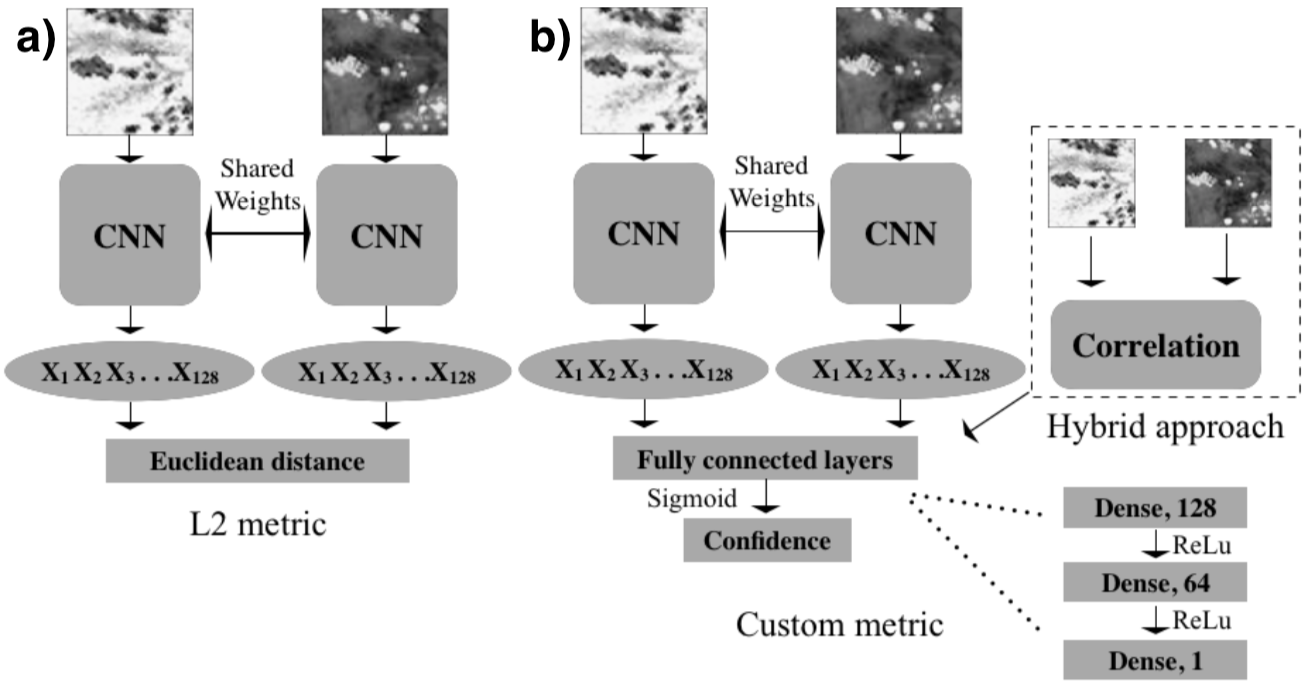
\includegraphics[width=130mm]{models.png}
     \caption{Архитектуры нейронных сетей для сопоставления изображений. a) дескрипторная сиамская сеть, b) попарная сиамская сеть}
     \label{graph}
\end{figure}

\end{document}